\chapter{Les ouvrages precedents sur les robot mobiles}
\section{Introduction}
nous allons exposer les principales recherches sur les robots autonomes, Nous allons adopter l'ordre chronologique, bien que certains travaux aient eu lieu en parallèle. On ne parlera pas des systèmes où le robot était astreint à suivre un chemin fixe déterminé par des équipements externes placés dans son environnement d'évolution On fera plutôt allusion aux travaux qui ont grandement aidé et marqué la nouvelle vague de robots mobiles dits de troisième génération.

\section{Le robot mobile SHAKEY:}
Shakey le robot est le premier robot générique capable de raisonner sur ses actions1. Il a été créé à la fin des années 1960 en Californie par SRI International avec le soutien de la DARPA. En 2004, il a été nommé au Robot Hall of Fame.\cite{ShakeyRobot2022}

Le robot Shakey pourrait analyser les commandes et les décomposer lui-même en morceaux de base. En raison de sa nature, le projet combinait des recherches en robotique, vision par ordinateur et traitement du langage naturel . Pour cette raison, c'était le premier projet qui mélangeait le raisonnement logique et l'action physique \cite{ShakyRobot}.

\newpage
\begin{figure}[h]
    \centering
    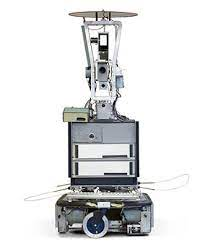
\includegraphics[width=10cm]{assets/Chapter2/ShakeyBot.jpeg}
    \caption{Le premier robot mobile SHAKEY \cite{ShakeyRobot2022}}
    \label{shakeybot}
    \end{figure}

En tant que précurseur, ce projet posa la plupart des problèmes conceptuels et y apporta des solutions intéressantes. Les problèmes techniques furent naturellement résolus avec les contraintes de la technologie de l'époque.

\subsection{Description du robot}
Le robot SHAKEY était symétrique possédant deux roues motrices.  L'axe des roues passait par le centre du robot, ces dernieres sont commandées par des moteurs indépendants et deux roues folles . Le robot avait la possibilité de ce deplacer en des lignes droites et des rotations autour de son axe vertical.

Le système de perception du robot est composé d'une caméra de type VISICON et un télémètre optique ainsi que des "moustaches de chat" , ce télémètre était utilisé comme détecteur de proximité.

La communication avec l'ordinateur de contrôle était assurée par deux liaisons radio dont une pour la transmission de l'image vidéo.

\newpage
\subsection{Systéme informatique du robot}
Le système du robot est passé par deux phases, initialement le système était constitué d’un ordinateur XDS-940 qui assurait toutes les taches mais ce système posait des problèmes sérieux de « swapping » entre les segments des différents programmes et de gestion d'interruptions en temps réel. Dans la deuxième phase, le 940 fut remplacé par un PDP-IO.
\subsection{Système décisionnel}
initialement le système était constitué d’un ordinateur XDS-940 qui assurait toutes les taches mais ce système posait des problèmes sérieux de « swapping » entre les segments des différents programmes et de gestion d'interruptions en temps réel. Apres, le 940 fut remplacé par un PDP-IO.

Au niveau le plus bas, se trouvaient les primitives du système qui permettaient la commande directe des effecteurs et senseurs.
Apres des actions de niveaux intermédiaires assuraient certaines fonctions comme la navigation. Ces actions étaient primitives du niveau supérieur STRIPS, les plans élaborés étaient exécutés par le niveau suivant, PLANEX.
Ce système décisionnel utilisait un seul modèle du monde  du calcul des prédicats du premier ordre. L'exécution des actions de bas niveau modifiait ce modèle du monde.
Des actions de niveau intermédiaire C'est le cas du système de navigation qui utilisait une grille plane de 4x4 carreaux, chaque cellule pouvait être:

(1) vide,
(2) pleine,
(3) partièlement pleine ou (4) de contenu inconnu
En tout trois niveaux de grille pouvaient être utilisés jusqu'à obtenir un carré d'un pied de côté. Un programme spécial avait pour tâche la mise à jour du conteur des cellules. Le modèle de grille était utilisé pour produire un graphe dont les noeuds (polyhedraux). Un arc liant deux noeuds indiquait que les deux sommets étaient atteignables  en ligne droite.
les noeuds étaient les sommets des obstacles grossis de manière à tenir compte de la taille du robot afin de le représenter par un point.
Le point représentatif du robot  et le meilleur chemin entre les deux points était fourni par l'utilisation de l'algorithme A* .
\newpage
\section{Le robot mobile JASON}
Le second projet de robot mobile complet fut celui de l'Université de Berkely. Le souci des concepteurs fut initiallement la limitation du coût.
\subsection{Desciption du véhicule}
Le robot était un véhicule de plusieurs étages mesurant 2x2x4 pieds et pesant 300 livres, et possédant deux roues motrice"s commandées par des moteurs à courant continu à l'arrière et une roue folle à l'avant.Un manipulateur de conception simple ainsi qu'une barre pour détecter le contact des objets et pour les pousser.
Les moyens de perceptions dont JASON fut effectivement doté consistaient en:
(i) une torche à ultrason à balayage qui devait permettre la mesure de la distance et de la texture des objets,(ii) 8 diodes électro-Iuminescentes en (LED) distribuées sur le pourtour du véhicule et sur détecteur de proximité.
\begin{figure}[h]
    \centering
    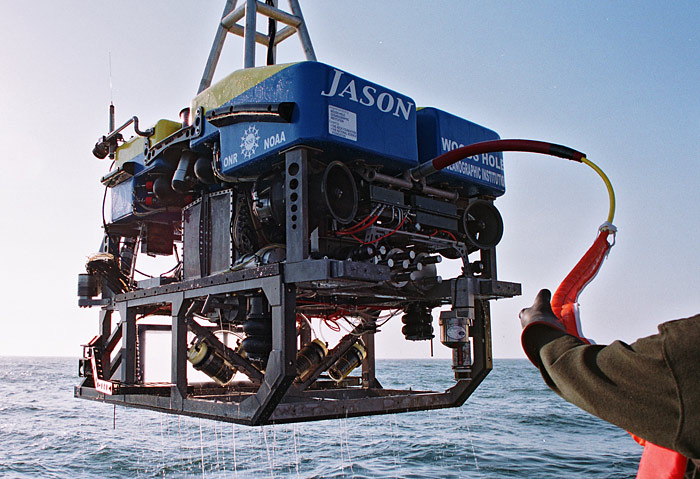
\includegraphics[width=14cm]{assets/Chapter2/jason1.jpeg}
    \caption{Le robot mobile JASON \cite{OceanRobotsJason}}
    \label{jason1}

\end{figure}

\subsection{Système décisionnel}
Ce système était initialement un miniordinateur HP3000 en temps partagé. Il fut ensuite remplacé par un PDPIO. L'emploi des microprocesseurs devenant de plus en plus courant, un projet d'un système multi- microprocesseur avec un Intel 8080 pour gérer chaque senseur fut étudié plus tard.
JASON pouvait être considéré comme un terminal ASCII pour le connecter à des ordinateurs différents.
\subsection{Système deécisionnel}
Ce système était composé de plusieurs "opérateurs" 
Le premier était conçu comme un réseau procédural dans lequel un graphe orienté des processus indiquait leurs conditions d'ordonnancement. Le second devait tenir compte des environnements ou l'information est incertaine, Deux modèles étaient utilisés par le système, Un modèle relationnel  et un modèle géométrique pour la navigation. Ce dernier consistait en une grille de taille et d'espacements de variables ramenée à un repère cartésien . Cette grille est remplie à partir des données du modèle relationnel sur la position et les dimensions des obstacles. . 
Les obstacles sont entourés d'une zone de sécurité égale à la moitié de la taille du robot afin de réduire ce dernier à un point.variables ramenée à un repère cartésien . 

Cette grille est remplie à partir des données du modèle relationnel sur la position et les dimensions des obstacles. . Les obstacles sont entourés d'une zone de sécurité égale à la moitié de la taille du robot afin de réduire ce dernier à un point.

La recherche de chemin, était effectuée en traçant la ligne droite qui joint le robot au but et en considérant l'une des extrémités des parois d'obstacle que coupe cette ligne comme sous- but, et ainsi de suite. Les capacités de manoeuvre de JASON posaient un problème particulier qui obligeaient soit à augmenter la taille de la zone de sécurité, soit à vérifier à chaque rotation et fin de ligne droite la possibilité d'une collision.

 
\section{Le robot mobile "ROVER"}
Le projet le plus ambitieux de robot mobile fut celui que le JPL a commencé à réaliser dans le but de mettre au point un système autonome d'exploration planétaire (pour la planète Mars). Ce robot devait donc évoluer dans un environnement "réaliste" (peu idéalisé) et être effectivement suffisamment performant puisque l'intervention de l'homme dans la boucle de décision ne pouvant être rapide (distances astronomiques...), ni parfois possible.
\begin{figure}[h]
    \centering
    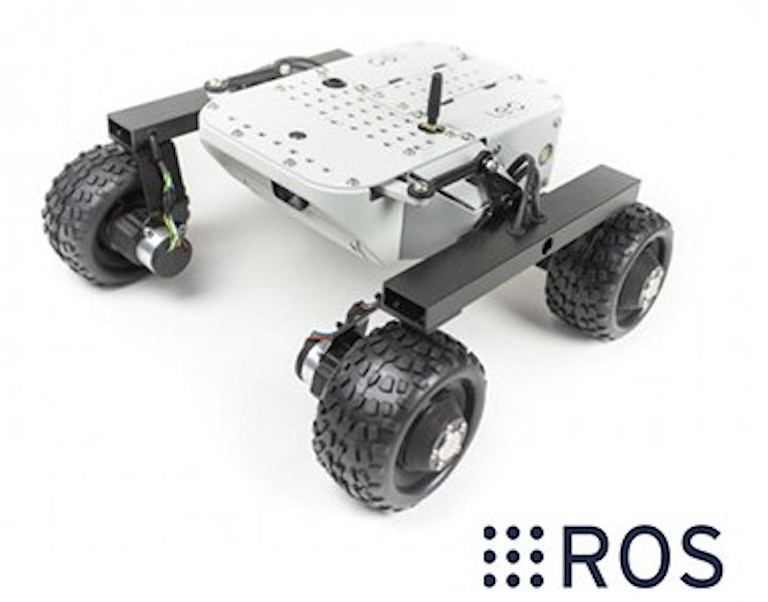
\includegraphics[width=8cm]{assets/Chapter2/rover.png}
    \caption{Le robot mobile Leo Rover }
    \label{roverbot}

\end{figure}

\newpage
\subsection{Description du véhicul}
Le robot expérimental servant de support de recherche était de la taille d'une petite voiture et comportait :
- un chassis avec 4 roues motrices, les paires avant et arrière pouvant tourner,

- divers capteurs de vitesse et d'attitude,


- 2 caméras et un télémètre laser,


- un manipulateur,


- une liaison radio.
\subsection{systéme Informatique}
Le système informatique devait être constitué par un réseau de microcalculateurs et un minicalculateur à bord, reliés à un gros ordinateur par radio. Le système a toutefois fonctionné initialement avec un minicalculateur GA SPC-16 et un PDPIO, en plus d'un système graphique IMLAC PDS-ID.
\subsection{Systéme décisionnel}

Il était conçu comme une hiérarchie de processus concurrents distribués sur les différents calculateurs. Ces processus pouvaient communiquer entre eux par un système de boîte aux lettres. La structure de contrôle principale à bord coordonnait plusieurs processus (vision, navigation, manipulation) et communiquait avec l'operateur à travers un système de contrôle "à terre".
Le système de navigation est constitué par 3 processus concou rents qui sont:
1) L'exécutif de la navigation;
2) Le module de planification du chemin; 3) Le module de contrôle du véhicule.
L'algorithme de recherche de chemin utilisé (PATH*) était similaire à A* et utilise la distance comme fonction de coût. Les chemins traversant des régions connues étaient préférés à ceux passant par des régions inconnues.
La taille et les capacités de manoeuvre du robot étaient prises en compte près des sommets en testant le chemin trouvé pour le centre. S'il y avait intersection entre les côtés des obstacles et la surface balayée par une translation du robot le long de ce chemin (les rotations sont aussi testées par une procédure particulière), on considérait les sommets du côté intersectant comme sous-buts,comme précédemment.
\newpage
\begin{figure}[h]
    \centering
    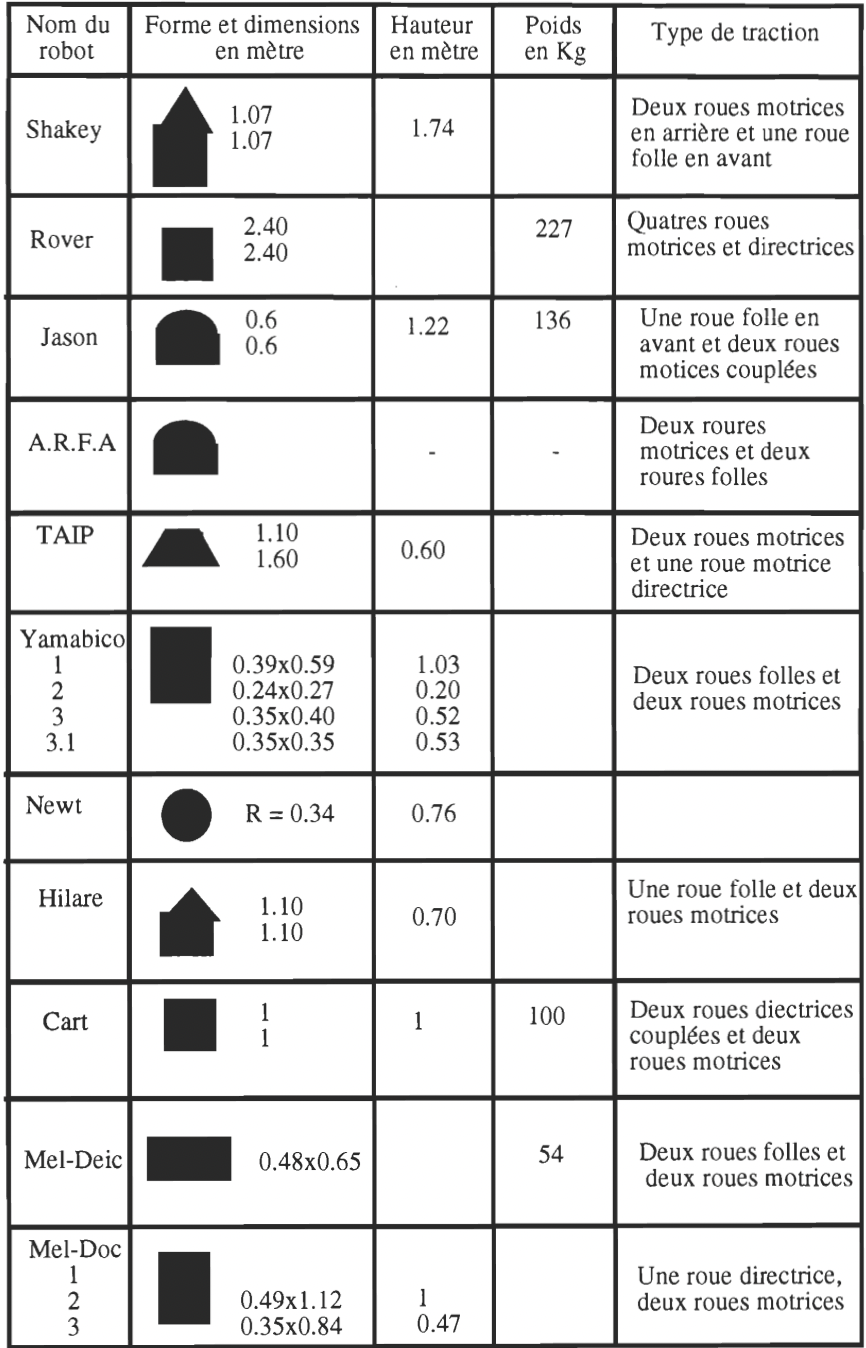
\includegraphics[width=14cm]{assets/Chapter2/chapitre2tab1.png}
    \caption{Tableau recapitulatif des robots (a)}
    \label{bottab1}

\end{figure}
\newpage
\begin{figure}[h]
    \centering
    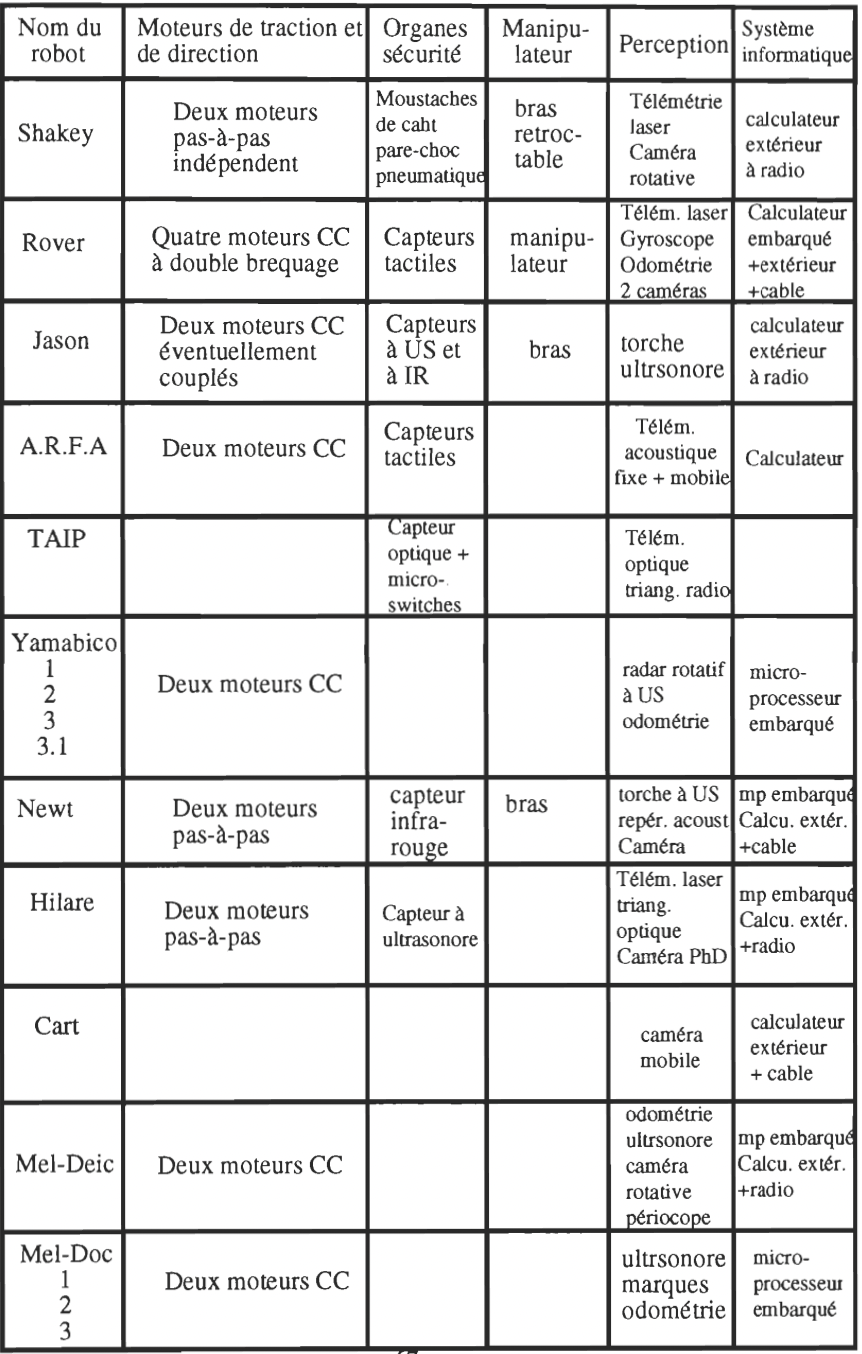
\includegraphics[width=14cm]{assets/Chapter2/chapitre2tab2.png}
    \caption{Tableau recapitulatif des robots (b)}
    \label{bottab2}

\end{figure}
\newpage
\section{Modélisation de la Caméra :}
\subsection{Conception}
Une caméra doit réaliser une transformation ponctuelle qui fait passer d’un point 
physique de l’espace réel 3D à un point 2D sur le plan image. Ce qui revient à une 
transformation mathématique de R3 vers R2.
Il existe plusieurs modèles dans la modélisation de la formation des images numériques. 
Notre étude prend comme modèle celui du sténopé ; appelé également le modèle perspectif 
(pin-hole en anglais) ; c'est un dispositif optique et le plus utilisé dans la vision par ordinateur. 
Ce modèle permet d'établir une relation entre un point de coordonnées 3D de la scène 
observée et sa projection dans l'image en 2D.
\subsection{ Composants d'une caméra :}
Une caméra se compose d'une boîte dont l'une de ses faces est percée d'un trou minuscule 
qui laisse entrer la lumière comme indique la figure (3.1). 
L'image vient se former sur la face opposée au trou et celle-ci peut être capturée en y 
plaçant un support photosensible (papier photographique).

image 

Une caméra perspective peut en effet être modélisée grâce au modèle du sténopé comme 
l'illustre la figure (3.2). Ce modèle associe à la caméra un repère cartésien ; ce repère dont son 
origine se situe sur le centre optique C est défini comme Rc = [Oc Xc Yc Zc ]. La caméra est 
représentée par un plan image, le plan image est parallèle aux axes Xc et Yc. Il est situé à une 
distance f de l'origine C appelée distance focale f de ce plan. La droite passant par le centre 
de projection et perpendiculaire au plan image est L'axe optique. L'intersection de l'axe 
optique avec le plan image est appelé point principal.

image

\section{Calibration D'une Caméra :}
Le calibrage consiste à estimer les paramètres intrinsèques et extrinsèques d'un modèle de 
caméra à partir d'un ensemble de points 3-D et de leur image. Il s'agit donc d'estimer les 
éléments de la matrice (3.7) ; Cette étape est incontournable pour de nombreuses applications 
de vision par l’ordinateur.Le calibrage de la caméra a été préalablement traité par la communauté de la 
photogrammétrie. Par conséquent, de nombreuses méthodes de calibrage ont été proposées
dans la littérature. Ces approches sont généralement classifiées en deux catégories :
\subsection{Calibrage avec un objet 3D de référence ou une mire :}
Cette technique utilise l’observation d’objets en 3D avec des coordonnées connues. Les 
objets de calibrage (mire) (figure (3.7)) sont généralement des points répartis sur des plans 
orthogonaux ou sur un plan translaté dans la direction de sa normale. Le calcul peut alors être 
effectué de façon relativement simple [dib11].
\subsection{Calibrage automatique (ou auto-calibrage) :}
Dans cette technique, Le mouvement connu de la caméra filmant une scène statique est 
utilisé pour poser des contraintes sur les paramètres intrinsèques prenant en compte la rigidité 
des objets filmés en utilisant uniquement les informations de l’image [dib11].
Nous avons opté pour la première famille ; sachant qu'elle est disponible sur internet " 
camera calibration toolbox for matlab". Elle consiste à calibrer la caméra à partir de 
plusieurs images d'une mire. Prises sous des points de vue différents comme indique la figure
(3.8).

image1
image2

Les positions des coins de chaque carré de la mire sont alors extraites puis raffinées en 
cas de distorsion. Ensuite les paramètres de la caméra sont déterminés par optimisation non 
linéaire.
\section{Résultat de la calibration de la caméra :}
Nous avons utilisé une webcam, type Logitech 720 hp (figure (3.9)) pour avoir un 
modèle et procéder à l'expérimentation. La caméra est placée sur un robot mobile qui se 
trouve au niveau du département d'électronique pour déterminer les paramètres intrinsèques 
de la caméra obtenus lors de la phase de calibrage. Leurs valeurs sont résumées dans le 
tableau (3.1).

image

tableau

La figure suivante présente le repère de la caméra Rc(Oc,Xc,Yc,Zc). La pyramide 
rouge correspond au champ de vue effectif de la caméra défini par le plan d'image.

image

Sur cette nouvelle figure, chaque position et orientation de la caméra sont représentées
par une pyramide verte par rapport à chaque image de calibration.
Estimation relative de la pose d'une caméra par rapport à chaque image de 
calibration.
%http://eprints.univ-batna2.dz/1125/1/ing%20Bouhamatou%20Zoulikha.pdf

image 

\section{ Définition des repères : }
La modélisation du robot s'appuie sur différents repères Figure (3.11) définis comme suit :
R(O,XY,Y: Le repère lié à la scène repère monde)
Rr(Or,Xr,Yr,Yr): Le repère lié à la base mobile
Rc(Oc,Xc,Yc,Yc): Le repère lié à la caméra

Pour la base mobile ; la position est représentée par les coordonnées (x,y) du point, Or dans le repère Rr tandis que l'orientation est donnée par l'angle T .la position de la caméra dans le repère est décrite par le vecteur Oc Or=(T,O,H).
Qb(X0,Y0,Z0,1): Un point de trajectoire est exprimé dans le repère monde. Sa projection 
dans le plan image est Q1(U1,V1,1) Alors, comme nous l'avons vu la relation :Q1=K*Tcb*Qb
Après calibrage, la matrice K est déterminée et le problème consiste ensuite à trouver la 
Tcb
La relation entre le point de l'espace dans le repère monde et repère caméra est :
Qc=Tcr*Trb*Qb
\section{Résultats de Simulations et discussion :}
Pour effectuer un asservissement visuel avec les paramètres obtenus, Nous avons 
procéder à une manipulation qui consiste à fournir au robot mobile les coordonnées 
échantillonnées d'une trajectoire que nous avons tracé sur une surface bien illuminée. Pour 
vérifier l'exactitude des coordonnées mesurées, nous avons choisi deux points sur la 
trajectoire à poursuivre en calculant leurs valeurs et les comparer avec celles mesurées (figure 
(3.13)). Les résultats de comparaison sont très satisfaisants et l'erreur est presque inexistante. 
 - la position de la caméra par rapport au repère monde est : 
[X,Y,Z]pow(r) = [20cm, 25cm, 30 cm]pow(T)
 -L'angle de rotation a été choisi entre le repère caméra et le repère monde.

 image tableau 
 \section{.Conclusion :}
 Après avoir présenté la partie calibrage et modélisation de la caméra nous avons procédé 
au calibrage d'une Webcam caméra que nous avons choisi en tenant compte du prix et de la 
qualité. Cette étape est nécessaire pour déterminer les paramètres intrinsèques et extrinsèques 
de la caméra. La modélisation de la caméra présente la projection du point de l'espace 3D à un 
point 2D sur le plan image par trois transformations élémentaire successives : la 
transformation rigide, la projection perspective et la transformation affine.



